\documentclass[12pt,a4paper]{article}
\usepackage[utf8]{inputenc}
\usepackage[portuguese]{babel}
\usepackage[T1]{fontenc}
\usepackage{graphicx}
\usepackage[left=2cm,right=2cm,top=2cm,bottom=2cm]{geometry}
\usepackage{indentfirst}
\usepackage{longtable}
\usepackage{tikz}
\usetikzlibrary{arrows,automata}




\begin{document}
\thispagestyle{empty}
\begin{center}
{\Large\sc Universidade Federal de Minas Gerais}

{\large Sistemas Digitais}

Prof. Julio Conway

\vfill
{\LARGE\bf Sistema de Destravamento Presencial Sequencial}

\medskip
Cleber Vargas Borges

Gabriel Machado de Castro Fonseca

\vfill
Belo Horizonte - MG

2015
\end{center}
\newpage

\section{Introdução}

A eletrônica talvez seja considerada o maior avanço tecnológico do século XX. A sua evolução se deu de forma exponencial, sendo hoje em dia uma tecnologia acessível e praticamente onipresente. Enquanto no início lidávamos com componentes grandes, delicados e pouco eficientes, com o passar das décadas, foram-se criando alternativas menores, menos dispendiosas e muito mais rápidas.

Com o uso da eletrônica digital e as possibilidades surgidas com a miniaturização dos circuitos, foi possível criar máquinas programáveis que cabem em nossos bolsos e executam milhões de cálculos a mais por segundo do que os primeiros computadores a válvulas. A lógica digital permite uma extrema maleabilidade na solução de um problema, fazendo com que blocos construtivos simples componham um circuito complexo, projetado para lidar com uma situação específica.

O objetivo deste trabalho é o de demonstrar a modelagem de um circuito lógico seqüencial que funcione como um sistema de destravamento de um cofre. São necessárias 3 pessoas para se abrir o cofre, cada uma deve digitar seu código de acesso na ordem certa para que a porta se destrave. Ao identificar corretamente a primeira pessoa uma luz vermelha se acende, a segunda pessoa a ser identificada faz com que se acenda uma luz amarela e, finalmente, quando a terceira pessoa é identificada acende-se uma luz verde e a tranca é aberta por 4 segundos, retornando então ao estado inicial. Qualquer erro de identificação ou na ordem de entrada das senhas faz com que se retorne ao estado inicial.

\section{Identificação dos Indivíduos}

Definimos que as senhas seriam, conforme instruções do trabalho, G0, C7 e J2. Conforme tabela ASCII, a representação das senhas, considerando maiúscula e minúscula, seria

\bigskip

\begin{table}[hb]
\begin{center}
\begin{tabular}{c||cccccccc|cccc}
Senha & $I_0$ & $I_1$ & $I_2$ & $I_3$ & $I_4$ & $I_5$ & $I_6$ & $I_7$ & $I_8$ & $I_9$ & $I_{10}$ & $I_{11}$ \\
\hline
G0 & {\bf 0} & {\bf 1} & {\bf 0} & 0 & 0 & 1 & 1 & 1 & {\bf 0} & 0 & 0 & 0 \\
g0 & {\bf 0} & {\bf 1} & {\bf 1} & 0 & 0 & 1 & 1 & 1 & {\bf 0} & 0 & 0 & 0 \\
\hline
\hline
C7 & {\bf 0} & {\bf 1} & {\bf 0} & 0 & 0 & 0 & 1 & 1 & {\bf 0} & 1 & 1 & 1 \\
c7 & {\bf 0} & {\bf 1} & {\bf 1} & 0 & 0 & 0 & 1 & 1 & {\bf 0} & 1 & 1 & 1 \\
\hline
\hline
J2 & {\bf 0} & {\bf 1} & {\bf 0} & 0 & 1 & 0 & 1 & 0 & {\bf 0} & 0 & 1 & 0 \\
j2 & {\bf 0} & {\bf 1} & {\bf 1} & 0 & 1 & 0 & 1 & 0 & {\bf 0} & 0 & 1 & 0 \\
\end{tabular}
\end{center}
\caption{Codificação ASCII das senhas do sistema}
\label{tab1}
\end{table}

Pode-se perceber que os números em destaque são redundantes para a identificação das senhas, uma vez que se repetem ou seguem um padrão óbvio, variando apenas um bit entre o caractere maiúsculo e minúsculo. Dessa forma podemos adotar apenas 6 bits para a letra e 3 bits para os números, uma vez que nenhuma senha possuí número maior que 8.

Na figura \ref{fig1} pode-se ver os circuitos lógicos necessários para se identificar as senhas da tabela \ref{tab1}.

\begin{figure}[!h]
\begin{center}
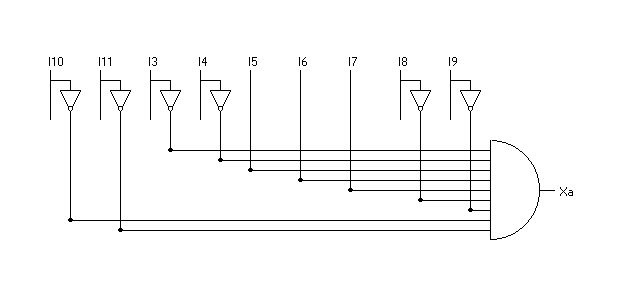
\includegraphics[width=.7\textwidth]{xa.png}
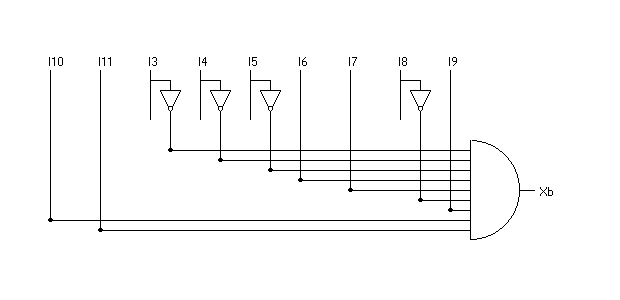
\includegraphics[width=.7\textwidth]{xb.png}
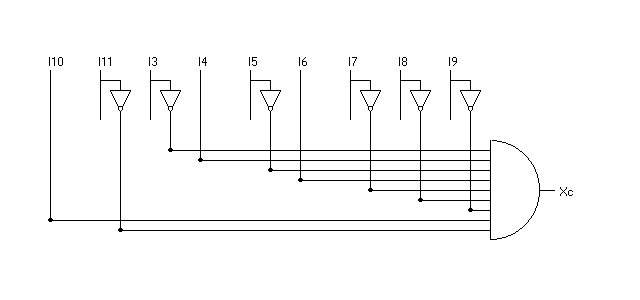
\includegraphics[width=.7\textwidth]{xc.png}
\end{center}
\caption{Lógica dos identificadores dos indivíduos}
\label{fig1}
\end{figure}

\section{Máquina de Estados Finitos}

O próximo passo da criação do sistema é a definição dos estados da máquina, para que possamos dimensionar as entradas, as saídas e as transições de estado, definindo em seguida o circuito lógico combinacional equivalente. Os estados da nossa máquina podem ser definidos conforme tabela \ref{tab2}. Com isso sabemos que os estados podem ser codificados usando 3 bits, que suportariam até 8 estados diferentes. A codificação deles pode ser vista na tabela \ref{tab3}.


\begin{table}[hb]
\begin{center}
\begin{tabular}{c|c|c}
\textbf{Estado} & \textbf{Descrição}\\ \hline
0 & Fechadura trancada, luzes apagadas, estado inicial \\
1 & Fechadura trancada, luz vermelha acesa \\
2 & Fechadura trancada, luzes vermelha e amarela acesas \\
3 & Fechadura destrancada, todas as luzes acesas \\
4 & Fechadura destrancada, todas as luzes acesas, 2 segundos passados \\
5 & Fechadura destrancada, todas as luzes acesas, 4 segundos passados \\ 
\hline
\end{tabular}
\end{center}
\caption{Descrição dos estados}
\label{tab2}
\end{table}


\begin{table}[!h]
\begin{tabular}{c|ccc}
Estado & $S_0$ & $S_1$ & $S_2$ \\ \hline
0 & 0 & 0 & 0 \\
1 & 0 & 0 & 1 \\
2 & 0 & 1 & 0 \\
3 & 0 & 1 & 1 \\
4 & 1 & 0 & 0 \\
5 & 1 & 0 & 1 \\
\end{tabular}
\label{tab3}
\end{table}

\begin{tikzpicture}[>=stealth',shorten >=1pt,auto,node distance=4cm]
  \node[initial,state] (0)      {0};
  \node[state]         (1) [right of=0]  {1};
  \node[state]         (2) [below right of=1] {2};
  \node[state]         (3) [below left of=2] {3};
  \node[state]         (4) [left of=3] {4};
  \node[state]         (5) [above left of=4] {5};

  \path[->] (0)  edge [loop above] node {$\overline{X_aX_b'X_c'}$} (0)
            edge              	node {$X_aX_b'X_c'$} (1)
        (1) edge [bend left]  	node {$\overline{X_aX_bX_c'}$} (0)
            edge              	node {$X_aX_bX_c'$} (2)
        (2) edge [bend left=45] node {$\overline{X_aX_bX_c}$} (0)
            edge              	node {$X_aX_bX_c$} (3)
        (3) edge				node {} (4)
        (4) edge				node {} (5)
        (5) edge				node {} (0);
\end{tikzpicture}

%\begin{table}[htbp]

\begin{longtable}{|ccc|ccc||ccc|c|c|c|}
\hline
\multicolumn{6}{|c|}{\textbf{Entradas}} & \multicolumn{6}{|c|}{\textbf{Saídas}} \\ \hline
\multicolumn{3}{|c|}{Identificadores} & \multicolumn{3}{|c|}{Est. Atual} & \multicolumn{3}{|c|}{Prox. Estado} & \multicolumn{3}{|c|}{Luzes} \\ \hline
$X_a$ & $X_b$ & $X_c$ & $S_0$ & $S_1$ & $S_2$ & $N_0$ & $N_1$ & $N_2$ & Vm & Am & Ve \\ \hline \endhead
0 & 0 & 0 & 0 & 0 & 0 & 0 & 0 & 0 & 0 & 0 & 0 \\ \hline
0 & 0 & 0 & 0 & 0 & 1 & 0 & 0 & 0 & 0 & 0 & 0 \\ \hline
0 & 0 & 0 & 0 & 1 & 0 & 0 & 0 & 0 & 0 & 0 & 0 \\ \hline
0 & 0 & 0 & 0 & 1 & 1 & 1 & 0 & 0 & 1 & 1 & 1 \\ \hline
0 & 0 & 0 & 1 & 0 & 0 & 1 & 0 & 1 & 1 & 1 & 1 \\ \hline
0 & 0 & 0 & 1 & 0 & 1 & 0 & 0 & 0 & 0 & 0 & 0 \\ \hline
0 & 0 & 0 & 1 & 1 & 0 & 0 & 0 & 0 & 0 & 0 & 0 \\ \hline
0 & 0 & 0 & 1 & 1 & 1 & 0 & 0 & 0 & 0 & 0 & 0 \\ \hline
0 & 0 & 1 & 0 & 0 & 0 & 0 & 0 & 0 & 0 & 0 & 0 \\ \hline
0 & 0 & 1 & 0 & 0 & 1 & 0 & 0 & 0 & 0 & 0 & 0 \\ \hline
0 & 0 & 1 & 0 & 1 & 0 & 0 & 0 & 0 & 0 & 0 & 0 \\ \hline
0 & 0 & 1 & 0 & 1 & 1 & 1 & 0 & 0 & 1 & 1 & 1 \\ \hline
0 & 0 & 1 & 1 & 0 & 0 & 1 & 0 & 1 & 1 & 1 & 1 \\ \hline
0 & 0 & 1 & 1 & 0 & 1 & 0 & 0 & 0 & 0 & 0 & 0 \\ \hline
0 & 0 & 1 & 1 & 1 & 0 & 0 & 0 & 0 & 0 & 0 & 0 \\ \hline
0 & 0 & 1 & 1 & 1 & 1 & 0 & 0 & 0 & 0 & 0 & 0 \\ \hline
0 & 1 & 0 & 0 & 0 & 0 & 0 & 0 & 0 & 0 & 0 & 0 \\ \hline
0 & 1 & 0 & 0 & 0 & 1 & 0 & 0 & 0 & 0 & 0 & 0 \\ \hline
0 & 1 & 0 & 0 & 1 & 0 & 0 & 0 & 0 & 0 & 0 & 0 \\ \hline
0 & 1 & 0 & 0 & 1 & 1 & 1 & 0 & 0 & 1 & 1 & 1 \\ \hline
0 & 1 & 0 & 1 & 0 & 0 & 1 & 0 & 1 & 1 & 1 & 1 \\ \hline
0 & 1 & 0 & 1 & 0 & 1 & 0 & 0 & 0 & 0 & 0 & 0 \\ \hline
0 & 1 & 0 & 1 & 1 & 0 & 0 & 0 & 0 & 0 & 0 & 0 \\ \hline
0 & 1 & 0 & 1 & 1 & 1 & 0 & 0 & 0 & 0 & 0 & 0 \\ \hline
0 & 1 & 1 & 0 & 0 & 0 & 0 & 0 & 0 & 0 & 0 & 0 \\ \hline
0 & 1 & 1 & 0 & 0 & 1 & 0 & 0 & 0 & 0 & 0 & 0 \\ \hline
0 & 1 & 1 & 0 & 1 & 0 & 0 & 0 & 0 & 0 & 0 & 0 \\ \hline
0 & 1 & 1 & 0 & 1 & 1 & 1 & 0 & 0 & 1 & 1 & 1 \\ \hline
0 & 1 & 1 & 1 & 0 & 0 & 1 & 0 & 1 & 1 & 1 & 1 \\ \hline
0 & 1 & 1 & 1 & 0 & 1 & 0 & 0 & 0 & 0 & 0 & 0 \\ \hline
0 & 1 & 1 & 1 & 1 & 0 & 0 & 0 & 0 & 0 & 0 & 0 \\ \hline
0 & 1 & 1 & 1 & 1 & 1 & 0 & 0 & 0 & 0 & 0 & 0 \\ \hline
1 & 0 & 0 & 0 & 0 & 0 & 0 & 0 & 1 & 1 & 0 & 0 \\ \hline
1 & 0 & 0 & 0 & 0 & 1 & 0 & 0 & 0 & 0 & 0 & 0 \\ \hline
1 & 0 & 0 & 0 & 1 & 0 & 0 & 0 & 0 & 0 & 0 & 0 \\ \hline
1 & 0 & 0 & 0 & 1 & 1 & 1 & 0 & 0 & 1 & 1 & 1 \\ \hline
1 & 0 & 0 & 1 & 0 & 0 & 1 & 0 & 1 & 1 & 1 & 1 \\ \hline
1 & 0 & 0 & 1 & 0 & 1 & 0 & 0 & 0 & 0 & 0 & 0 \\ \hline
1 & 0 & 0 & 1 & 1 & 0 & 0 & 0 & 0 & 0 & 0 & 0 \\ \hline
1 & 0 & 0 & 1 & 1 & 1 & 0 & 0 & 0 & 0 & 0 & 0 \\ \hline
1 & 0 & 1 & 0 & 0 & 0 & 0 & 0 & 0 & 0 & 0 & 0 \\ \hline
1 & 0 & 1 & 0 & 0 & 1 & 0 & 0 & 0 & 0 & 0 & 0 \\ \hline
1 & 0 & 1 & 0 & 1 & 0 & 0 & 0 & 0 & 0 & 0 & 0 \\ \hline
1 & 0 & 1 & 0 & 1 & 1 & 1 & 0 & 0 & 1 & 1 & 1 \\ \hline
1 & 0 & 1 & 1 & 0 & 0 & 1 & 0 & 1 & 1 & 1 & 1 \\ \hline
1 & 0 & 1 & 1 & 0 & 1 & 0 & 0 & 0 & 0 & 0 & 0 \\ \hline
1 & 0 & 1 & 1 & 1 & 0 & 0 & 0 & 0 & 0 & 0 & 0 \\ \hline
1 & 0 & 1 & 1 & 1 & 1 & 0 & 0 & 0 & 0 & 0 & 0 \\ \hline
1 & 1 & 0 & 0 & 0 & 0 & 0 & 0 & 0 & 0 & 0 & 0 \\ \hline
1 & 1 & 0 & 0 & 0 & 1 & 0 & 1 & 0 & 1 & 1 & 0 \\ \hline
1 & 1 & 0 & 0 & 1 & 0 & 0 & 0 & 0 & 0 & 0 & 0 \\ \hline
1 & 1 & 0 & 0 & 1 & 1 & 1 & 0 & 0 & 1 & 1 & 1 \\ \hline
1 & 1 & 0 & 1 & 0 & 0 & 1 & 0 & 1 & 1 & 1 & 1 \\ \hline
1 & 1 & 0 & 1 & 0 & 1 & 0 & 0 & 0 & 0 & 0 & 0 \\ \hline
1 & 1 & 0 & 1 & 1 & 0 & 0 & 0 & 0 & 0 & 0 & 0 \\ \hline
1 & 1 & 0 & 1 & 1 & 1 & 0 & 0 & 0 & 0 & 0 & 0 \\ \hline
1 & 1 & 1 & 0 & 0 & 0 & 0 & 0 & 0 & 0 & 0 & 0 \\ \hline
1 & 1 & 1 & 0 & 0 & 1 & 0 & 0 & 0 & 0 & 0 & 0 \\ \hline
1 & 1 & 1 & 0 & 1 & 0 & 0 & 1 & 1 & 1 & 1 & 1 \\ \hline
1 & 1 & 1 & 0 & 1 & 1 & 1 & 0 & 0 & 1 & 1 & 1 \\ \hline
1 & 1 & 1 & 1 & 0 & 0 & 1 & 0 & 1 & 1 & 1 & 1 \\ \hline
1 & 1 & 1 & 1 & 0 & 1 & 0 & 0 & 0 & 0 & 0 & 0 \\ \hline
1 & 1 & 1 & 1 & 1 & 0 & 0 & 0 & 0 & 0 & 0 & 0 \\ \hline
1 & 1 & 1 & 1 & 1 & 1 & 0 & 0 & 0 & 0 & 0 & 0 \\ \hline

\caption{Tabela verdade da máquina de estados}
\label{tabV}
\end{longtable}
%\end{table}


\end{document}